% \iffalse meta-comment
%
% Copyright (C) 2021 by Diego Arcis <arcisd@gmail.com>
% --------------------------------------------------------------------
% This work may be distributed and/or modified under the conditions of
% the LaTeX Project Public License, either version 1.3 of this license
% or (at your option) any later version.
%
% The latest version of this license is in:
% 	http://www.latex-project.org/lppl.txt
%
% and version 1.3 or later is part of all distributions of LaTeX, that
% is, version 2005/12/01 or later.
%
% The Current Maintainer of this work is Diego Arcis.
%
% This work consists of the files strands.dtx and strands.ins and they
% derive the filebase strands.sty.
% --------------------------------------------------------------------
%
% \fi
%
% \iffalse
%<package>\NeedsTeXFormat{LaTeX2e}[2005/12/01]
%<package>\ProvidesPackage{strands}[2021/07/11 v1.1 Strands]
%
%<*driver>
\documentclass{ltxdoc}
\usepackage{strands}
\EnableCrossrefs
\CodelineIndex
\RecordChanges
\begin{document}
	\DocInput{strands.dtx}
\end{document}
%</driver>
% \fi
%
% \CheckSum{1713}
%
% \CharacterTable
%  {Upper-case    \A\B\C\D\E\F\G\H\I\J\K\L\M\N\O\P\Q\R\S\T\U\V\W\X\Y\Z
%   Lower-case    \a\b\c\d\e\f\g\h\i\j\k\l\m\n\o\p\q\r\s\t\u\v\w\x\y\z
%   Digits        \0\1\2\3\4\5\6\7\8\9
%   Exclamation   \!     Double quote  \"     Hash (number) \#
%   Dollar        \$     Percent       \%     Ampersand     \&
%   Acute accent  \'     Left paren    \(     Right paren   \)
%   Asterisk      \*     Plus          \+     Comma         \,
%   Minus         \-     Point         \.     Solidus       \/
%   Colon         \:     Semicolon     \;     Less than     \<
%   Equals        \=     Greater than  \>     Question mark \?
%   Commercial at \@     Left bracket  \[     Backslash     \\
%   Right bracket \]     Circumflex    \^     Underscore    \_
%   Grave accent  \`     Left brace    \{     Vertical bar  \|
%   Right brace   \}     Tilde         \~}
%
%
% \changes{v1.1}{2021/07/11}{Initial version}
%
% \GetFileInfo{strands.sty}
%
% \DoNotIndex{\#,\$,\%,\&,\@,\\,\{,\},\^,\_,\~,\}
% \DoNotIndex{\@ne}
% \DoNotIndex{\advance,\begingroup,\catcode,\closein}
% \DoNotIndex{\closeout,\day,\def,\edef,\else,\empty,\endgroup}
%
% \title{The \textsf{strands} package
%   \thanks{This document corresponds to \textsf{strands}~\fileversion, dated~\filedate.}
% }
% \author{Diego Arcis \\ \texttt{arcisd@gmail.com}}
%
% \maketitle
%
% \StopEventually{\PrintIndex}

% packages:
\RequirePackage{forarray}
\RequirePackage{ifthen}
\RequirePackage{tikz}
\RequirePackage{xfp}
\RequirePackage{xstring}
\RequirePackage{xkeyval}

\usetikzlibrary{snakes}

\newcommand{\getelem}[3]{ % \getelem{list}{index}{\name}
	\StrBetween[#2,\fpeval{#2+1}]{,#1,}{,}{,}[#3]
}

% global variables:
\makeatletter
\define@cmdkey[str]{strands}{backcolor}{}
\define@cmdkey[str]{strands}{bend}{}
\define@cmdkey[str]{strands}{bendbraid}{}
\define@cmdkey[str]{strands}{bendtangle}{}
\define@cmdkey[str]{strands}{bulletsize}{}
\define@cmdkey[str]{strands}{braidcross}{}
\define@cmdkey[str]{strands}{braidsingcross}{}
\define@cmdkey[str]{strands}{braidvirtcross}{}
\define@cmdkey[str]{strands}{coverunion}{}
\define@cmdkey[str]{strands}{direction}{}
\define@cmdkey[str]{strands}{externalize}{}
\define@cmdkey[str]{strands}{font}{}
\define@cmdkey[str]{strands}{gencharposbraid}{}
\define@cmdkey[str]{strands}{gencharnegbraid}{}
\define@cmdkey[str]{strands}{gencharvirtual}{}
\define@cmdkey[str]{strands}{gencharsingular}{}
\define@cmdkey[str]{strands}{genchartangle}{}
\define@cmdkey[str]{strands}{genchartie}{}
\define@cmdkey[str]{strands}{genchartiedtangle}{}
\define@cmdkey[str]{strands}{genchartrivial}{}
\define@cmdkey[str]{strands}{height}{}
\define@cmdkey[str]{strands}{labelver}{}
\define@cmdkey[str]{strands}{labelhor}{}
\define@cmdkey[str]{strands}{norma}{}
\define@cmdkey[str]{strands}{normb}{}
\define@cmdkey[str]{strands}{normcolor}{}
\define@cmdkey[str]{strands}{normsymbol}{}
\define@cmdkey[str]{strands}{nstr}{}
\define@cmdkey[str]{strands}{num}{}
\define@cmdkey[str]{strands}{rotate}{}
\define@cmdkey[str]{strands}{scale}{}
\define@cmdkey[str]{strands}{strwidth}{}
\define@cmdkey[str]{strands}{tiebend}{}
\define@cmdkey[str]{strands}{tiebull}{}
\define@cmdkey[str]{strands}{tiebullsize}{}
\define@cmdkey[str]{strands}{tiecolor}{}
\define@cmdkey[str]{strands}{tieheight}{}
\define@cmdkey[str]{strands}{tiesnake}{}
\define@cmdkey[str]{strands}{tiesnakeamp}{}
\define@cmdkey[str]{strands}{tiesnakends}{}
\define@cmdkey[str]{strands}{tiesnakelen}{}
\define@cmdkey[str]{strands}{tiestyle}{}
\define@cmdkey[str]{strands}{tiewidth}{}
\define@cmdkey[str]{strands}{timeswidth}{}
\define@cmdkey[str]{strands}{tkzpic}{}
\define@cmdkey[str]{strands}{width}{}

% default options:
\presetkeys[str]{strands}{
	backcolor=white, % color of the paper.
	bend=45, % bend of partitions.
	bendbraid=30, % bend for braid crossings.
	bendtangle=45, % bend for tangles.
	braidcross=3, % size of the braid crossing.
	braidsingcross=1.6, % size of the singular braid crossing.
	braidvirtcross=8, % size of the virtual braid crossing.
	bulletsize=0.04,
	coverunion=0.001, % extra length to cover the union of strands.
	direction=1,
	externalize=0, % use 1 to transform images to PDF.
	font=0.7, % size of the fonts for labels.
	gencharposbraid=p,
	gencharnegbraid=n,
	gencharvirtual=v,
	gencharsingular=s,
	genchartangle=t,
	genchartie=e,
	genchartiedtangle=f,
	genchartrivial=i,
	height=1, % to set the height of strands.
	labelver=0.2,
	labelhor=0.03,
	norma=0, % to normalize the height above.
	normb=0, % to normalize the height below.
	normcolor=transparent,
	normsymbol=-,
	nstr=0, % number of strands.
	num=0, % number of dots for arc partitions.
	rotate=0, % to rotate all pictures.
	scale=1, % to scale all pictures.
	strwidth=0.7, % to set the width of the strands.
	tiebend=0, % to set bend of ties.
	tiebull=0, % bullets for ties.
	tiebullsize=0.04,
	tiecolor=red, % to set color of the ties.
	tieheight=0.5, % height of ties respect to the global height.
	tiesnake=false,
	tiesnakeamp=1,
	tiesnakends=0,
	tiesnakelen=3,
	tiestyle=dashed, % to set the type of the tie lines.
	tiewidth=0.5, % to set the width of tie lines.
	timeswidth=3,
	tkzpic=1,
	width=0.6, % to set the width between strands.
}{}

\setkeys[str]{strands}{}

% declare custom options:
\DeclareOptionX{backcolor}{\renewcommand{\cmdstr@strands@backcolor}{#1}}
\DeclareOptionX{bend}{\renewcommand{\cmdstr@strands@bend}{#1}}
\DeclareOptionX{bendbraid}{\renewcommand{\cmdstr@strands@bendbraid}{#1}}
\DeclareOptionX{bendtangle}{\renewcommand{\cmdstr@strands@bendtangle}{#1}}
\DeclareOptionX{braidcross}{\renewcommand{\cmdstr@strands@braidcross}{#1}}
\DeclareOptionX{braidsingcross}{\renewcommand{\cmdstr@strands@braidsingcross}{#1}}
\DeclareOptionX{braidvirtcross}{\renewcommand{\cmdstr@strands@braidvirtcross}{#1}}
\DeclareOptionX{bulletsize}{\renewcommand{\cmdstr@strands@bulletsize}{#1}}
\DeclareOptionX{coverunion}{\renewcommand{\cmdstr@strands@coverunion}{#1}}
\DeclareOptionX{direction}{\renewcommand{\cmdstr@strands@direction}{#1}}
\DeclareOptionX{externalize}{\renewcommand{\cmdstr@strands@externalize}{#1}}
\DeclareOptionX{font}{\renewcommand{\cmdstr@strands@font}{#1}}
\DeclareOptionX{gencharposbraid}{\renewcommand{\cmdstr@strands@gencharposbraid}{#1}}
\DeclareOptionX{gencharnegbraid}{\renewcommand{\cmdstr@strands@gencharnegbraid}{#1}}
\DeclareOptionX{gencharvirtual}{\renewcommand{\cmdstr@strands@gencharvirtual}{#1}}
\DeclareOptionX{gencharsingular}{\renewcommand{\cmdstr@strands@gencharsingular}{#1}}
\DeclareOptionX{genchartangle}{\renewcommand{\cmdstr@strands@genchartangle}{#1}}
\DeclareOptionX{genchartie}{\renewcommand{\cmdstr@strands@genchartie}{#1}}
\DeclareOptionX{genchartiedtangle}{\renewcommand{\cmdstr@strands@genchartiedtangle}{#1}}
\DeclareOptionX{height}{\renewcommand{\cmdstr@strands@height}{#1}}
\DeclareOptionX{labelver}{\renewcommand{\cmdstr@strands@labelver}{#1}}
\DeclareOptionX{labelhor}{\renewcommand{\cmdstr@strands@labelhor}{#1}}
\DeclareOptionX{norma}{\renewcommand{\cmdstr@strands@norma}{#1}}
\DeclareOptionX{normb}{\renewcommand{\cmdstr@strands@normb}{#1}}
\DeclareOptionX{normcolor}{\renewcommand{\cmdstr@strands@normcolor}{#1}}
\DeclareOptionX{nstr}{\renewcommand{\cmdstr@strands@nstr}{#1}}
\DeclareOptionX{num}{\renewcommand{\cmdstr@strands@num}{#1}}
\DeclareOptionX{rotate}{\renewcommand{\cmdstr@strands@rotate}{#1}}
\DeclareOptionX{scale}{\renewcommand{\cmdstr@strands@scale}{#1}}
\DeclareOptionX{strwidth}{\renewcommand{\cmdstr@strands@strwidth}{#1}}
\DeclareOptionX{tiebend}{\renewcommand{\cmdstr@strands@tiebend}{#1}}
\DeclareOptionX{tiebull}{\renewcommand{\cmdstr@strands@tiebull}{#1}}
\DeclareOptionX{tiebullsize}{\renewcommand{\cmdstr@strands@tiebullsize}{#1}}
\DeclareOptionX{tiecolor}{\renewcommand{\cmdstr@strands@tiecolor}{#1}}
\DeclareOptionX{tiesnake}{\renewcommand{\cmdstr@strands@tiesnake}{#1}}
\DeclareOptionX{tiestyle}{\renewcommand{\cmdstr@strands@tiestyle}{#1}}
\DeclareOptionX{tiewidth}{\renewcommand{\cmdstr@strands@tiewidth}{#1}}
\DeclareOptionX{timeswidth}{\renewcommand{\cmdstr@strands@timeswidth}{#1}}
\DeclareOptionX{tkzpic}{\renewcommand{\cmdstr@strands@tkzpic}{#1}}
\DeclareOptionX{width}{\renewcommand{\cmdstr@strands@width}{#1}}
\DeclareOptionX*{\PackageWarning{strands}{`\CurrentOption' ignored}} % ignore unknown options.
\ProcessOptionsX\relax

\ifnum\cmdstr@strands@externalize=1
	\usetikzlibrary{external}
	\tikzexternalize[optimize=false,prefix=strpack]
\fi

% \decoratestrands - macro to add bullets and labels to picture.

\makeatletter
\define@cmdkey[str]{decor}{bulla}{}
\define@cmdkey[str]{decor}{bullb}{}
\define@cmdkey[str]{decor}{bulletends}{}
\define@cmdkey[str]{decor}{floor}{}
\define@cmdkey[str]{decor}{font}{}
\define@cmdkey[str]{decor}{height}{}
\define@cmdkey[str]{decor}{labelver}{}
\define@cmdkey[str]{decor}{labelhor}{}
\define@cmdkey[str]{decor}{nstr}{}
\define@cmdkey[str]{decor}{type}{}
\define@cmdkey[str]{decor}{width}{}

\presetkeys[str]{decor}{
	bulla=1,
	bullb=1,
	bulletends=\cmdstr@strands@bulletsize,
	floor=0,
	font=\cmdstr@strands@font,
	height=\cmdstr@strands@height,
	labelver=\cmdstr@strands@labelver,
	labelhor=\cmdstr@strands@labelhor,
	nstr=\cmdstr@strands@nstr,
	type=3,
	width=\cmdstr@strands@width
}{}

\newcommand{\decoratestrands}[1][]{
	\setkeys[str]{decor}{#1} % set variables.
	\foreach\ind in{0,...,\fpeval{\cmdstr@decor@nstr-1}}{
		\ifnum \cmdstr@decor@bulla=1 % bullets above.
			\filldraw(\fpeval{\ind*\cmdstr@decor@width},
			\fpeval{(\cmdstr@decor@floor+1)*\cmdstr@decor@height})circle(\cmdstr@decor@bulletends);
		\fi
		\ifnum \cmdstr@decor@bullb=1 % bullets below.
			\filldraw(\fpeval{\ind*\cmdstr@decor@width},
			\fpeval{\cmdstr@decor@floor*\cmdstr@decor@height})circle(\cmdstr@decor@bulletends);
		\fi
		% classic labels.
		\ifnum \cmdstr@decor@type<5;
			\ifnum \cmdstr@decor@type>0 % labels above from 1 to n.
				\node[scale=\cmdstr@decor@font]at
					(\fpeval{\ind*\cmdstr@decor@width},
					\fpeval{(\cmdstr@decor@floor+1)*\cmdstr@decor@height+\cmdstr@decor@labelver})
					{$\fpeval{\ind+1}$};
			\fi
			\node[scale=\cmdstr@decor@font]at
				(\fpeval{\ind*\cmdstr@decor@width},
				\fpeval{\cmdstr@decor@floor*\cmdstr@decor@height-\cmdstr@decor@labelver})
				{$\ifnum\fpeval{(\cmdstr@decor@type+1)*(\cmdstr@decor@type-2)}=0{
					\fpeval{\ind+1}
				}\else{\ifnum\fpeval{abs(\cmdstr@decor@type)}=3{
					\fpeval{\ind+\cmdstr@decor@nstr+1}
				}\else{\ifnum\fpeval{abs(\cmdstr@decor@type)}=4{
					\fpeval{\ind+1}'
				}\fi}\fi}\fi$};
		\fi
		% signed labels (n must be even).
		\ifnum \cmdstr@decor@type=5
			\ifnum\ind<\fpeval{\cmdstr@decor@nstr/2} % labels from -2n to 2n.
				\node[scale=\cmdstr@decor@font]at
					(\fpeval{(\ind+\cmdstr@decor@nstr/2)*\cmdstr@decor@width},
					\fpeval{(\cmdstr@decor@floor+1)*\cmdstr@decor@height+\cmdstr@decor@labelver})
					{$\fpeval{\ind+1}$};
				\node[scale=\cmdstr@decor@font]at
					(\fpeval{\ind*\cmdstr@decor@width-\cmdstr@decor@labelhor},
					\fpeval{(\cmdstr@decor@floor+1)*\cmdstr@decor@height+\cmdstr@decor@labelver})
					{-$\fpeval{\cmdstr@decor@nstr/2-\ind}$};
				\node[scale=\cmdstr@decor@font]at
					(\fpeval{(\ind+\cmdstr@decor@nstr/2)*\cmdstr@decor@width},
					\fpeval{\cmdstr@decor@floor*\cmdstr@decor@height-\cmdstr@decor@labelver})
					{$\fpeval{\ind+\cmdstr@decor@nstr/2+1}$};
				\node[scale=\cmdstr@decor@font]at
					(\fpeval{\ind*\cmdstr@decor@width-\cmdstr@decor@labelhor},
					\fpeval{\cmdstr@decor@floor*\cmdstr@decor@height-\cmdstr@decor@labelver})
					{-$\fpeval{\cmdstr@decor@nstr-\ind}$};
			\fi
		\fi
	}
}

% \vpartition  - macro to draw set partitions in the partition monoid.

% Example: the set partition {1,2}{3,-4}{4,-3} of [2*4] is drawn as follows: 

% \vpartition[<options>]{{1,2},{3,-4},{4,-3}}

%  1   2   3   4
%  |   |   |   |
%  -----    - -
%            -
%           - -
%          |   |
%  5   6   7   8

\makeatletter
\define@cmdkey[str]{vvpart}{bend}{}
\define@cmdkey[str]{vvpart}{bulla}{}
\define@cmdkey[str]{vvpart}{bullb}{}
\define@cmdkey[str]{vvpart}{bulletends}{}
\define@cmdkey[str]{vvpart}{floor}{}
\define@cmdkey[str]{vvpart}{font}{}
\define@cmdkey[str]{vvpart}{height}{}
\define@cmdkey[str]{vvpart}{labelver}{}
\define@cmdkey[str]{vvpart}{labelhor}{}
\define@cmdkey[str]{vvpart}{norma}{}
\define@cmdkey[str]{vvpart}{normb}{}
\define@cmdkey[str]{vvpart}{nstr}{}
\define@cmdkey[str]{vvpart}{permut}{}
\define@cmdkey[str]{vvpart}{reflect}{}
\define@cmdkey[str]{vvpart}{strwidth}{}
\define@cmdkey[str]{vvpart}{type}{}
\define@cmdkey[str]{vvpart}{width}{}

\presetkeys[str]{vvpart}{
	bend=\cmdstr@strands@bend,
	bulla=1,
	bullb=1,
	bulletends=\cmdstr@strands@bulletsize,
	floor=0,
	font=\cmdstr@strands@font,
	height=\cmdstr@strands@height,
	labelver=\cmdstr@strands@labelver,
	labelhor=\cmdstr@strands@labelhor,
	norma=\cmdstr@strands@norma,
	normb=\cmdstr@strands@normb,
	nstr=\cmdstr@strands@nstr,
	permut=0, % use 1 to draw permutations (to use with \permutation).
	reflect=0,
	strwidth=\cmdstr@strands@strwidth,
	type=3,
	width=\cmdstr@strands@width
}{}

\newcommand{\vvpartition}[2][]{
	\setkeys[str]{vvpart}{#1} % set variables.
	% normalize vertical size.
	\node[\cmdstr@strands@normcolor]at(0,\cmdstr@vvpart@norma){\cmdstr@strands@normsymbol};
	\node[\cmdstr@strands@normcolor]at(0,\cmdstr@vvpart@normb){\cmdstr@strands@normsymbol};
	% number of strands.
	\StrRemoveBraces{#2}[\nobracespart]
	\let\oldnumstrands\cmdstr@vvpart@nstr
	\renewcommand{\cmdstr@vvpart@nstr}
	{\fpeval{max(abs(min(\nobracespart)),abs(max(\nobracespart)),\fpeval{abs(\oldnumstrands)})}}
	% bullets and labels.
	\decoratestrands[
		bulla=\cmdstr@vvpart@bulla,
		bullb=\cmdstr@vvpart@bullb,
		bulletends=\cmdstr@vvpart@bulletends,
		floor=\cmdstr@vvpart@floor,
		font=\cmdstr@vvpart@font,
		height=\cmdstr@vvpart@height,
		labelver=\cmdstr@vvpart@labelver,
		labelhor=\cmdstr@vvpart@labelhor,
		nstr=\cmdstr@vvpart@nstr,
		type=\cmdstr@vvpart@type,
		width=\cmdstr@vvpart@width
	]
	% connections: permutation case.
	\foreach\ind in{0,...,\fpeval{\cmdstr@vvpart@nstr-1}}{
		\ifnum\cmdstr@vvpart@permut=1
			\getelem{#2}{\fpeval{\ind+1}}{\index} 
			\draw[line width=\cmdstr@vvpart@strwidth](\fpeval{\ind*\cmdstr@vvpart@width},
				\fpeval{\cmdstr@vvpart@height+\cmdstr@vvpart@floor*\cmdstr@vvpart@height})to
				(\fpeval{(\ifnum\fpeval{\index+0}>0 \index\else\fpeval{\ind+1}\fi-1)*
				\cmdstr@vvpart@width},\cmdstr@vvpart@floor*\cmdstr@vvpart@height);
		\fi
	}
	% connections: general case.
	\ifnum\cmdstr@vvpart@permut=0 \foreach\block in{#2}{
		\StrCount{\block}{,}[\numcom]
		\ifnum\numcom>0\foreach\ind in {2,...,\fpeval{\numcom+1}}{
			\getelem{\block}{\fpeval{\ind-1}}{\firbul}
			\getelem{\block}{\ind}{\secbul}
			\ifnum \cmdstr@vvpart@reflect=1 % reflect connections vertically.
				\let\oldfirbul\firbul
				\renewcommand{\firbul}{-\oldfirbul}
				\let\oldsecbul\secbul
				\renewcommand{\secbul}{-\oldsecbul}
			\fi
			\draw[line width=\cmdstr@vvpart@strwidth]
				% from.
				(\fpeval{(abs(\firbul)-1)*\cmdstr@vvpart@width},
					\ifnum\firbul>0 
						\fpeval{(\cmdstr@vvpart@floor+1)*\cmdstr@vvpart@height}
					\else
						\fpeval{\cmdstr@vvpart@floor*\cmdstr@vvpart@height}
					\fi
				)
					% bending.
					to[bend right=\ifnum \fpeval{\firbul*\secbul}>0
						\fpeval{(\firbul/abs(\firbul))*((abs(\secbul)-abs(\firbul))/
						abs(abs(\secbul)-abs(\firbul)))*\cmdstr@vvpart@bend}
					\else
						0
					\fi]
				% to.
				(\fpeval{(abs(\secbul)-1)*\cmdstr@vvpart@width},
					\ifnum\secbul>0
						\fpeval{(\cmdstr@vvpart@floor+1)*\cmdstr@vvpart@height}
					\else
						\fpeval{\cmdstr@vvpart@floor*\cmdstr@vvpart@height}
					\fi
				);
		}\fi
	}\fi
}

\makeatletter
\define@cmdkey[str]{vpart}{bend}{}
\define@cmdkey[str]{vpart}{bulla}{}
\define@cmdkey[str]{vpart}{bullb}{}
\define@cmdkey[str]{vpart}{bulletends}{}
\define@cmdkey[str]{vpart}{floor}{}
\define@cmdkey[str]{vpart}{font}{}
\define@cmdkey[str]{vpart}{height}{}
\define@cmdkey[str]{vpart}{labelver}{}
\define@cmdkey[str]{vpart}{labelhor}{}
\define@cmdkey[str]{vpart}{norma}{}
\define@cmdkey[str]{vpart}{normb}{}
\define@cmdkey[str]{vpart}{nstr}{}
\define@cmdkey[str]{vpart}{permut}{}
\define@cmdkey[str]{vpart}{reflect}{}
\define@cmdkey[str]{vpart}{rotate}{}
\define@cmdkey[str]{vpart}{scale}{}
\define@cmdkey[str]{vpart}{strwidth}{}
\define@cmdkey[str]{vpart}{tkzpic}{}
\define@cmdkey[str]{vpart}{type}{}
\define@cmdkey[str]{vpart}{width}{}

\presetkeys[str]{vpart}{
	bend=\cmdstr@strands@bend,
	bulla=1,
	bullb=1,
	bulletends=\cmdstr@strands@bulletsize,
	floor=0,
	font=\cmdstr@strands@font,
	height=\cmdstr@strands@height,
	labelver=\cmdstr@strands@labelver,
	labelhor=\cmdstr@strands@labelhor,
	norma=\cmdstr@strands@norma,
	normb=\cmdstr@strands@normb,
	nstr=\cmdstr@strands@nstr,
	permut=0, % use 1 to draw permutations (to use with \permutation).
	reflect=0,
	rotate=\cmdstr@strands@rotate,
	scale=\cmdstr@strands@scale,
	strwidth=\cmdstr@strands@strwidth,
	tkzpic=\cmdstr@strands@tkzpic,
	type=3,
	width=\cmdstr@strands@width
}{}

\newcommand{\vpartition}[2][]{
	\setkeys[str]{vpart}{#1} % set variables.
	\ifthenelse{\equal{\cmdstr@vpart@tkzpic}{1}}{
		\begin{tikzpicture}[rotate=\cmdstr@vpart@rotate,scale=\cmdstr@vpart@scale]
			\vvpartition[
				bend=\cmdstr@vpart@bend,
				bulla=\cmdstr@vpart@bulla,
				bullb=\cmdstr@vpart@bullb,
				bulletends=\cmdstr@vpart@bulletends,
				floor=\cmdstr@vpart@floor,
				font=\cmdstr@vpart@font,
				height=\cmdstr@vpart@height,
				labelver=\cmdstr@vpart@labelver,
				labelhor=\cmdstr@vpart@labelhor,
				norma=\cmdstr@vpart@norma,
				normb=\cmdstr@vpart@normb,
				nstr=\cmdstr@vpart@nstr,
				permut=\cmdstr@vpart@permut,
				reflect=\cmdstr@vpart@reflect,
				strwidth=\cmdstr@vpart@strwidth,
				type=\cmdstr@vpart@type,
				width=\cmdstr@vpart@width
			]{#2}
		\end{tikzpicture}
	}{
		\vvpartition[
			bend=\cmdstr@vpart@bend,
			bulla=\cmdstr@vpart@bulla,
			bullb=\cmdstr@vpart@bullb,
			bulletends=\cmdstr@vpart@bulletends,
			floor=\cmdstr@vpart@floor,
			font=\cmdstr@vpart@font,
			height=\cmdstr@vpart@height,
			labelver=\cmdstr@vpart@labelver,
			labelhor=\cmdstr@vpart@labelhor,
			norma=\cmdstr@vpart@norma,
			normb=\cmdstr@vpart@normb,
			nstr=\cmdstr@vpart@nstr,
			permut=\cmdstr@vpart@permut,
			reflect=\cmdstr@vpart@reflect,
			strwidth=\cmdstr@vpart@strwidth,
			type=\cmdstr@vpart@type,
			width=\cmdstr@vpart@width
		]{#2}
	}
}


% \arcpartition  - macro to draw set partitions via arcs.

% Example: the set partition {1,4}{2,3,7} of [7] is drawn as follows: 

% \arcpartition[<options>]{{1,4},{2,3,7}}

%          -----------------
%          |               |
%  -------------           |
%  |       |   |           |
%  |   -----   |           |
%  |   |   |   |           |
%  1   2   3   4   5   6   7

\makeatletter
\define@cmdkey[str]{apart}{bend}{}
\define@cmdkey[str]{apart}{bull}{}
\define@cmdkey[str]{apart}{bulletsize}{}
\define@cmdkey[str]{apart}{floor}{}
\define@cmdkey[str]{apart}{font}{}
\define@cmdkey[str]{apart}{labelver}{}
\define@cmdkey[str]{apart}{labelhor}{}
\define@cmdkey[str]{apart}{norma}{}
\define@cmdkey[str]{apart}{normb}{}
\define@cmdkey[str]{apart}{num}{}
\define@cmdkey[str]{apart}{rotate}{}
\define@cmdkey[str]{apart}{scale}{}
\define@cmdkey[str]{apart}{strwidth}{}
\define@cmdkey[str]{apart}{tkzpic}{}
\define@cmdkey[str]{apart}{type}{}
\define@cmdkey[str]{apart}{width}{}

\presetkeys[str]{apart}{
	bend=\cmdstr@strands@bend,
	bull=1,
	bulletsize=\cmdstr@strands@bulletsize,
	floor=0,
	font=\cmdstr@strands@font,
	labelver=\cmdstr@strands@labelver,
	labelhor=\cmdstr@strands@labelhor,
	norma=\cmdstr@strands@norma,
	normb=\cmdstr@strands@normb,
	num=\cmdstr@strands@num,
	rotate=\cmdstr@strands@rotate,
	scale=\cmdstr@strands@scale,
	strwidth=\cmdstr@strands@strwidth,
	tkzpic=\cmdstr@strands@tkzpic,
	type=1,
	width=\cmdstr@strands@width
}{}

\newcommand{\arcpartition}[2][]{
	\setkeys[str]{apart}{#1}
	\vpartition[
		bend=\cmdstr@apart@bend,
		bulla=0, % no bullets above.
		bullb=\cmdstr@apart@bull,
		bulletends=\cmdstr@apart@bulletsize,
		floor=\cmdstr@apart@floor,
		font=\cmdstr@apart@font,
		labelver=\cmdstr@apart@labelver,
		labelhor=\cmdstr@apart@labelhor,
		norma=\cmdstr@apart@norma,
		normb=\cmdstr@apart@normb,
		nstr=\cmdstr@apart@num,
		reflect=1, % put connections below.
		rotate=\cmdstr@apart@rotate,
		scale=\cmdstr@apart@scale,
		strwidth=\cmdstr@apart@strwidth,
		tkzpic=\cmdstr@apart@tkzpic,
		type=-\cmdstr@apart@type,
		width=\cmdstr@apart@width
	]{#2}
}

% \permutation  - macro to draw permutations by lines.

% Example: the permutation 2134 of [4] is drawn as follows: 

% \permutation[<options>]{2,1,3,4}

%  1   2   3   4
%  |   |   |   |
%   - -    |   |
%    -     |   |
%   - -    |   |
%  |   |   |   |
%  1   2   3   4

\makeatletter
\define@cmdkey[str]{perm}{bulla}{}
\define@cmdkey[str]{perm}{bullb}{}
\define@cmdkey[str]{perm}{bulletends}{}
\define@cmdkey[str]{perm}{floor}{}
\define@cmdkey[str]{perm}{font}{}
\define@cmdkey[str]{perm}{height}{}
\define@cmdkey[str]{perm}{labelver}{}
\define@cmdkey[str]{perm}{labelhor}{}
\define@cmdkey[str]{perm}{norma}{}
\define@cmdkey[str]{perm}{normb}{}
\define@cmdkey[str]{perm}{nstr}{}
\define@cmdkey[str]{perm}{rotate}{}
\define@cmdkey[str]{perm}{scale}{}
\define@cmdkey[str]{perm}{strwidth}{}
\define@cmdkey[str]{perm}{tkzpic}{}
\define@cmdkey[str]{perm}{type}{}
\define@cmdkey[str]{perm}{width}{}

\presetkeys[str]{perm}{
	bulla=1,
	bullb=1,
	bulletends=\cmdstr@strands@bulletsize,
	floor=0,
	font=\cmdstr@strands@font,
	height=\cmdstr@strands@height,
	labelver=\cmdstr@strands@labelver,
	labelhor=\cmdstr@strands@labelhor,
	norma=\cmdstr@strands@norma,
	normb=\cmdstr@strands@normb,
	nstr=\cmdstr@strands@nstr,
	rotate=\cmdstr@strands@rotate,
	scale=\cmdstr@strands@scale,
	strwidth=\cmdstr@strands@strwidth,
	tkzpic=\cmdstr@strands@tkzpic,
	type=2,
	width=\cmdstr@strands@width
}{}

\newcommand{\permutation}[2][]{
	\setkeys[str]{perm}{#1}
	\vpartition[
		bulla=\cmdstr@perm@bulla,
		bullb=\cmdstr@perm@bullb,
		bulletends=\cmdstr@perm@bulletends,
		floor=\cmdstr@perm@floor,
		font=\cmdstr@perm@font,
		height=\cmdstr@perm@height,
		labelver=\cmdstr@perm@labelver,
		labelhor=\cmdstr@perm@labelhor,
		norma=\cmdstr@perm@norma,
		normb=\cmdstr@perm@normb,
		nstr=\cmdstr@perm@nstr,
		permut=1, % permutation.
		rotate=\cmdstr@perm@rotate,
		scale=\cmdstr@perm@scale,
		strwidth=\cmdstr@perm@strwidth,
		tkzpic=\cmdstr@perm@tkzpic,
		type=\cmdstr@perm@type,
		width=\cmdstr@perm@width
	]{#2}
}

% \tiedpair - macro to draw a tied permutation as a pair.

% Example: the permutation ({2,4},2134) of [4] is drawn as follows:

% \tiedpair[<options>]{{2,4}}{2,1,3,4}

%      2       4
%      ---------
%  1   |   3   |
%  |   |   |   |
%   - -    |   |
%    -     |   |
%   - -    |   |
%  |   |   |   |
%  1   2   3   4

\makeatletter
\define@cmdkey[str]{tpair}{above}{}
\define@cmdkey[str]{tpair}{bend}{}
\define@cmdkey[str]{tpair}{bulla}{}
\define@cmdkey[str]{tpair}{bullb}{}
\define@cmdkey[str]{tpair}{bulletends}{}
\define@cmdkey[str]{tpair}{floor}{}
\define@cmdkey[str]{tpair}{font}{}
\define@cmdkey[str]{tpair}{height}{}
\define@cmdkey[str]{tpair}{labelver}{}
\define@cmdkey[str]{tpair}{labelhor}{}
\define@cmdkey[str]{tpair}{norma}{}
\define@cmdkey[str]{tpair}{normb}{}
\define@cmdkey[str]{tpair}{nstr}{}
\define@cmdkey[str]{tpair}{rotate}{}
\define@cmdkey[str]{tpair}{scale}{}
\define@cmdkey[str]{tpair}{strwidth}{}
\define@cmdkey[str]{tpair}{tkzpic}{}
\define@cmdkey[str]{tpair}{type}{}
\define@cmdkey[str]{tpair}{width}{}

\presetkeys[str]{tpair}{
	above=1,
	bend=\cmdstr@strands@bend,
	bulla=1,
	bullb=1,
	bulletends=\cmdstr@strands@bulletsize,
	floor=0,
	font=\cmdstr@strands@font,
	height=\cmdstr@strands@height,
	labelver=\cmdstr@strands@labelver,
	labelhor=\cmdstr@strands@labelhor,
	norma=\cmdstr@strands@norma,
	normb=\cmdstr@strands@normb,
	nstr=\cmdstr@strands@nstr,
	rotate=\cmdstr@strands@rotate,
	scale=\cmdstr@strands@scale,
	strwidth=\cmdstr@strands@strwidth,
	tkzpic=\cmdstr@strands@tkzpic,
	type=-1,
	width=\cmdstr@strands@width
}{}

\newcommand{\tiedpair}[3][]{
	\setkeys[str]{tpair}{#1}
	\ifthenelse{\equal{\cmdstr@tpair@tkzpic}{1}}{
		\begin{tikzpicture}[rotate=\cmdstr@tpair@rotate,scale=\cmdstr@tpair@scale]
			\permutation[
				bulla=\cmdstr@tpair@bulla,
				bullb=\cmdstr@tpair@bullb,
				bulletends=\cmdstr@tpair@bulletends,
				floor=\cmdstr@tpair@floor,
				font=\cmdstr@tpair@font,
				height=\cmdstr@tpair@height,
				labelver=\cmdstr@tpair@labelver,
				labelhor=\cmdstr@tpair@labelhor,
				norma=\cmdstr@tpair@norma,
				normb=\cmdstr@tpair@normb,
				nstr=\cmdstr@tpair@nstr,
				strwidth=\cmdstr@tpair@strwidth,
				tkzpic=0,
				type=\cmdstr@tpair@type,
				width=\cmdstr@tpair@width
			]{#2}
			\arcpartition[
				bend=\cmdstr@tpair@bend,
				bull=0, % no bullets.
				bulletsize=\cmdstr@tpair@bulletsize,
				floor=\fpeval{\cmdstr@tpair@floor+\cmdstr@tpair@above*\cmdstr@tpair@height},
				tkzpic=0,
				type=0, % no labels.
				strwidth=\cmdstr@tpair@strwidth,
				width=\cmdstr@tpair@width
			]{#3}
		\end{tikzpicture}
	}{
		\permutation[
			bulla=\cmdstr@tpair@bulla,
			bullb=\cmdstr@tpair@bullb,
			bulletends=\cmdstr@tpair@bulletends,
			floor=\cmdstr@tpair@floor,
			font=\cmdstr@tpair@font,
			height=\cmdstr@tpair@height,
			labelver=\cmdstr@tpair@labelver,
			labelhor=\cmdstr@tpair@labelhor,
			norma=\cmdstr@tpair@norma,
			normb=\cmdstr@tpair@normb,
			nstr=\cmdstr@tpair@nstr,
			strwidth=\cmdstr@tpair@strwidth,
			tkzpic=0,
			type=\cmdstr@tpair@type,
			width=\cmdstr@tpair@width
		]{#2}
		\arcpartition[
			bend=\cmdstr@tpair@bend,
			bull=0, % no bullets.
			floor=\fpeval{\cmdstr@tpair@floor+\cmdstr@tpair@above*\cmdstr@tpair@height},
			tkzpic=0,
			type=0, % no labels.
			strwidth=\cmdstr@tpair@strwidth,
			width=\cmdstr@tpair@width
		]{#3}
	}
}

% \tie  - macro to draw a tie.

% 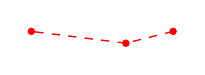
\begin{tikzpicture} \tie[height=1.5]{{1,0.8},{3,0.7},{4,0.8}} \end{tikzpicture}
% \begin{tikzpicture} \tie[height=1.5]{1,2,5} \end{tikzpicture}

\makeatletter
\define@cmdkey[str]{tie}{bend}{}
\define@cmdkey[str]{tie}{bull}{}
\define@cmdkey[str]{tie}{bulletie}{}
\define@cmdkey[str]{tie}{floor}{}
\define@cmdkey[str]{tie}{height}{}
\define@cmdkey[str]{tie}{color}{}
\define@cmdkey[str]{tie}{snake}{}
\define@cmdkey[str]{tie}{snakeamp}{}
\define@cmdkey[str]{tie}{snakends}{}
\define@cmdkey[str]{tie}{snakelen}{}
\define@cmdkey[str]{tie}{style}{}
\define@cmdkey[str]{tie}{tieheight}{}
\define@cmdkey[str]{tie}{tiewidth}{}
\define@cmdkey[str]{tie}{width}{}

\presetkeys[str]{tie}{
	bend=\cmdstr@strands@tiebend, % bend of the ties.
	bull=1, % use 1 to use bullets, 0 otherwise.
	bulletie=\cmdstr@strands@bulletsize,
	color=\cmdstr@strands@tiecolor, % color of the ties.
	floor=0, % the picture starts at floor*height.
	height=\cmdstr@strands@height, % height of the strands.
	snake=\cmdstr@strands@tiesnake, % true or false to snake the tie line.
	snakeamp=\cmdstr@strands@tiesnakeamp, % snake amplitude.
	snakends=\cmdstr@strands@tiesnakends, % snake lengths of ends.
	snakelen=\cmdstr@strands@tiesnakelen, % snake lengths.
	style=\cmdstr@strands@tiestyle, % type of the tie (solid, dashed, dotted, etc).
	tieheight=\cmdstr@strands@tieheight, % height of the tie respect to the global height.
	tiewidth=\cmdstr@strands@tiewidth, % width of the tie line.
	width=\cmdstr@strands@width % width between strands.
}{}

\newcommand{\tie}[2][]{
	\setkeys[str]{tie}{#1}
	\foreach\elem[count=\ind]in{#2}{
		\StrRemoveBraces{\elem}[\nobrace]
		\getelem{\nobrace}{1}{\elemwidth} % get width of elem.
		\getelem{\nobrace}{2}{\elemheight} % get height of elem.
		\StrCount{\nobrace}{,}[\elemcoms]
		\ifnum\elemcoms=0 \renewcommand{\elemheight}{\cmdstr@tie@tieheight}\fi % update height of elem.
		\ifnum \cmdstr@tie@bull=1
			\filldraw[\cmdstr@tie@color](\fpeval{(\elemwidth-1)*\cmdstr@tie@width},
				\fpeval{\elemheight*\cmdstr@tie@height+\cmdstr@tie@floor*\cmdstr@tie@height})
				circle(\cmdstr@tie@bulletie);
		\fi
		\ifnum\ind>1
			\getelem{#2}{\fpeval{\ind-1}}{\prevelem}
			\StrRemoveBraces{\prevelem}[\prevnobrace]
			\getelem{\prevnobrace}{1}{\prevelemwidth}
			\getelem{\prevnobrace}{2}{\prevelemheight}
			\StrCount{\prevnobrace}{,}[\prevelemcoms]
			\ifnum\prevelemcoms=0 \renewcommand{\prevelemheight}{\cmdstr@tie@tieheight}\fi
			\draw[
				bend right=\cmdstr@tie@bend,
				color=\cmdstr@tie@color,
				line width=\cmdstr@tie@tiewidth,
				decorate=\cmdstr@tie@snake,
				decoration={
					snake,
					amplitude=\cmdstr@tie@snakeamp,
					post length=\cmdstr@tie@snakends,
					pre length=\cmdstr@tie@snakends,
					segment length=\cmdstr@tie@snakelen
				},
				style=\cmdstr@tie@style
			]
				(\fpeval{(\elemwidth-1)*\cmdstr@tie@width},
				\fpeval{\elemheight*\cmdstr@tie@height+\cmdstr@tie@floor*\cmdstr@tie@height})to
				(\fpeval{(\prevelemwidth-1)*\cmdstr@tie@width},
				\fpeval{\prevelemheight*\cmdstr@tie@height+\cmdstr@tie@floor*\cmdstr@tie@height});
		\fi
	}
}

% \bbackstrands - macro to draws a trivial two-strands-braid of double strand width.

\makeatletter
\define@cmdkey[str]{bbackstr}{cdnx}{}
\define@cmdkey[str]{bbackstr}{cdny}{}
\define@cmdkey[str]{bbackstr}{color}{}
\define@cmdkey[str]{bbackstr}{height}{}
\define@cmdkey[str]{bbackstr}{strwidth}{}
\define@cmdkey[str]{bbackstr}{timeswidth}{}
\define@cmdkey[str]{bbackstr}{width}{}

\presetkeys[str]{bbackstr}{
	cdnx=nothing,
	cdny=nothing,
	height=\cmdstr@strands@height,
	strwidth=\cmdstr@strands@strwidth,
	timeswidth=\cmdstr@strands@timeswidth, % times the width of the back line is bigger.
	width=\cmdstr@strands@width
}{}

\newcommand{\bbackstrands}[1][]{ % 
	\setkeys[str]{bbackstr}{#1}
	\draw[
		color=\cmdstr@strands@backcolor,
		line width=\fpeval{\cmdstr@bbackstr@timeswidth*\cmdstr@bbackstr@strwidth}pt
	](\cmdstr@bbackstr@cdnx,\cmdstr@bbackstr@cdny)
	to(\cmdstr@bbackstr@cdnx,\fpeval{\cmdstr@bbackstr@cdny-\cmdstr@bbackstr@height});
	\draw[
		color=\cmdstr@strands@backcolor,
		line width=\fpeval{\cmdstr@bbackstr@timeswidth*\cmdstr@bbackstr@strwidth}pt
	](\fpeval{\cmdstr@bbackstr@cdnx+\cmdstr@bbackstr@width},\cmdstr@bbackstr@cdny)
	to(\fpeval{\cmdstr@bbackstr@cdnx+\cmdstr@bbackstr@width},
		\fpeval{\cmdstr@bbackstr@cdny-\cmdstr@bbackstr@height});
}

% \lleftstrand - macro to draws a strand starting from the left.

\makeatletter
\define@cmdkey[str]{lleftstr}{bend}{}
\define@cmdkey[str]{lleftstr}{cdnx}{}
\define@cmdkey[str]{lleftstr}{cdny}{}
\define@cmdkey[str]{lleftstr}{color}{}
\define@cmdkey[str]{lleftstr}{height}{}
\define@cmdkey[str]{lleftstr}{strwidth}{}
\define@cmdkey[str]{lleftstr}{width}{}

\presetkeys[str]{lleftstr}{
	bend=\cmdstr@strands@bendbraid,
	cdnx=nothing,
	cdny=nothing,
	color=black,
	height=\cmdstr@strands@height,
	strwidth=\cmdstr@strands@strwidth,
	width=\cmdstr@strands@width
}{}

\newcommand{\lleftstrand}[1][]{
	\setkeys[str]{lleftstr}{#1}
	\draw[
		color=\cmdstr@lleftstr@color,
		line width=\cmdstr@lleftstr@strwidth pt
	](\cmdstr@lleftstr@cdnx,\fpeval{\cmdstr@lleftstr@cdny+\cmdstr@strands@coverunion})
	to[bend right=\cmdstr@lleftstr@bend]
		(\fpeval{\cmdstr@lleftstr@cdnx+\cmdstr@lleftstr@width/2},
		\fpeval{\cmdstr@lleftstr@cdny-\cmdstr@lleftstr@height/2})
	to[bend left=\cmdstr@lleftstr@bend]
		(\fpeval{\cmdstr@lleftstr@cdnx+\cmdstr@lleftstr@width},
		\fpeval{\cmdstr@lleftstr@cdny-\cmdstr@lleftstr@height-\cmdstr@strands@coverunion});
}

% \rrightstrand - macro to draw a strand starting from the right.

\makeatletter
\define@cmdkey[str]{rrightstr}{bend}{}
\define@cmdkey[str]{rrightstr}{cdnx}{}
\define@cmdkey[str]{rrightstr}{cdny}{}
\define@cmdkey[str]{rrightstr}{color}{}
\define@cmdkey[str]{rrightstr}{floor}{}
\define@cmdkey[str]{rrightstr}{height}{}
\define@cmdkey[str]{rrightstr}{strwidth}{}
\define@cmdkey[str]{rrightstr}{width}{}

\presetkeys[str]{rrightstr}{
	bend=\cmdstr@strands@bendbraid,
	cdnx=nothing,
	cdny=nothing,
	color=black,
	floor=0,
	height=\cmdstr@strands@height,
	strwidth=\cmdstr@strands@strwidth,
	width=\cmdstr@strands@width
}{}

\newcommand{\rrightstrand}[1][]{ % color / init-x-coordinate / init-y-coordinate.
	\setkeys[str]{rrightstr}{#1}
	\draw[
		color=\cmdstr@rrightstr@color,
		line width=\cmdstr@rrightstr@strwidth pt
	](\fpeval{\cmdstr@rrightstr@cdnx+\cmdstr@rrightstr@width},
		\fpeval{\cmdstr@rrightstr@cdny+\cmdstr@strands@coverunion})
	to[bend left=\cmdstr@rrightstr@bend]
		(\fpeval{\cmdstr@rrightstr@cdnx+\cmdstr@rrightstr@width/2},
		\fpeval{\cmdstr@rrightstr@cdny-\cmdstr@rrightstr@height/2})
	to[bend right=\cmdstr@rrightstr@bend]
		(\cmdstr@rrightstr@cdnx,
		\fpeval{\cmdstr@rrightstr@cdny-\cmdstr@rrightstr@height-\cmdstr@strands@coverunion});
}

% \ccrossback - macro to draw a \backcolor filled circle to create an over-under / under-over crossing.

\makeatletter
\define@cmdkey[str]{ccrossback}{cdnx}{}
\define@cmdkey[str]{ccrossback}{cdny}{}
\define@cmdkey[str]{ccrossback}{height}{}
\define@cmdkey[str]{ccrossback}{width}{}

\presetkeys[str]{ccrossback}{
	cdnx=nothing,
	cdny=nothing,
	height=\cmdstr@strands@height,
	width=\cmdstr@strands@width
}{}

\newcommand{\ccrossback}[1][]{
	\setkeys[str]{ccrossback}{#1}
	\filldraw[\cmdstr@strands@backcolor]
		(\fpeval{\cmdstr@ccrossback@cdnx+\cmdstr@ccrossback@width/2},
		\fpeval{\cmdstr@ccrossback@cdny-\cmdstr@ccrossback@height/2})
		circle(\cmdstr@strands@braidcross pt);
}

% \bbraidgen - macro to draw a braid crossing (classic, virtual or singular).

\makeatletter
\define@cmdkey[str]{bbraidgen}{bend}{}
\define@cmdkey[str]{bbraidgen}{cdnx}{}
\define@cmdkey[str]{bbraidgen}{cdny}{}
\define@cmdkey[str]{bbraidgen}{colorleft}{}
\define@cmdkey[str]{bbraidgen}{coloright}{}
\define@cmdkey[str]{bbraidgen}{colorsingular}{}
\define@cmdkey[str]{bbraidgen}{colorvirtual}{}
\define@cmdkey[str]{bbraidgen}{height}{}
\define@cmdkey[str]{bbraidgen}{strwidth}{}
\define@cmdkey[str]{bbraidgen}{type}{}
\define@cmdkey[str]{bbraidgen}{width}{}

\presetkeys[str]{bbraidgen}{
	bend=\cmdstr@strands@bendbraid,
	cdnx=0,
	cdny=0,
	colorleft=black,
	coloright=black,
	colorsingular=black,
	colorvirtual=black,
	height=\cmdstr@strands@height,
	strwidth=\cmdstr@strands@strwidth,
	type=1, % negative-braid=-1 | positive-braid=1 | virtual-braid=2 | singular-braid=3
	width=\cmdstr@strands@width
}{}

\tikzset{
	cross/.style={ % node style to draw x--crosses inside nodes.
		path picture={
  			\draw[black]
				(path picture bounding box.south east)--
				(path picture bounding box.north west)
				(path picture bounding box.south west)--
				(path picture bounding box.north east);
		}
	}
}

\newcommand{\bbraidgen}[1][]{
	\setkeys[str]{bbraidgen}{#1}
	\bbackstrands[ % trivial two-strands-braid.
		cdnx=\cmdstr@bbraidgen@cdnx,
		cdny=\cmdstr@bbraidgen@cdny,
		height=\cmdstr@bbraidgen@height,
		strwidth=\cmdstr@bbraidgen@strwidth,
		width=\cmdstr@bbraidgen@width
	]
	\ifnum\cmdstr@bbraidgen@type<1 % negative generator.
		\rrightstrand[
			bend=\cmdstr@bbraidgen@bend,
			cdnx=\cmdstr@bbraidgen@cdnx,
			cdny=\cmdstr@bbraidgen@cdny,
			color=\cmdstr@bbraidgen@coloright,
			height=\cmdstr@bbraidgen@height,
			strwidth=\cmdstr@bbraidgen@strwidth,
			width=\cmdstr@bbraidgen@width
		]
		\ifnum\cmdstr@bbraidgen@type<2
			\ccrossback[
				cdnx=\cmdstr@bbraidgen@cdnx,
				cdny=\cmdstr@bbraidgen@cdny,
				height=\cmdstr@bbraidgen@height,
				width=\cmdstr@bbraidgen@width
			]
		\fi
		\lleftstrand[
			bend=\cmdstr@bbraidgen@bend,
			cdnx=\cmdstr@bbraidgen@cdnx,
			cdny=\cmdstr@bbraidgen@cdny,
			color=\cmdstr@bbraidgen@colorleft,
			height=\cmdstr@bbraidgen@height,
			strwidth=\cmdstr@bbraidgen@strwidth,
			width=\cmdstr@bbraidgen@width
		]
	\else % positive generator.
		\lleftstrand[
			bend=\cmdstr@bbraidgen@bend,
			cdnx=\cmdstr@bbraidgen@cdnx,
			cdny=\cmdstr@bbraidgen@cdny,
			color=\cmdstr@bbraidgen@colorleft,
			height=\cmdstr@bbraidgen@height,
			strwidth=\cmdstr@bbraidgen@strwidth,
			width=\cmdstr@bbraidgen@width
		]
		\ifnum\cmdstr@bbraidgen@type<2 % over-under circle only if type is one.
			\ccrossback[
				cdnx=\cmdstr@bbraidgen@cdnx,
				cdny=\cmdstr@bbraidgen@cdny,
				height=\cmdstr@bbraidgen@height,
				width=\cmdstr@bbraidgen@width
			]
		\fi
		\rrightstrand[
			bend=\cmdstr@bbraidgen@bend,
			cdnx=\cmdstr@bbraidgen@cdnx,
			cdny=\cmdstr@bbraidgen@cdny,
			color=\cmdstr@bbraidgen@coloright,
			height=\cmdstr@bbraidgen@height,
			strwidth=\cmdstr@bbraidgen@strwidth,
			width=\cmdstr@bbraidgen@width
		]
		\ifnum\cmdstr@bbraidgen@type=2 % virtual crossing.
			\node[
				circle,
				cross,
				draw=\cmdstr@bbraidgen@colorvirtual,
				fill=\cmdstr@strands@backcolor,
				inner sep=0,
				line width=\cmdstr@bbraidgen@strwidth,
				minimum width=\cmdstr@strands@braidvirtcross
			]
			at(\fpeval{\cmdstr@bbraidgen@cdnx+\cmdstr@bbraidgen@width/2},
				\fpeval{\cmdstr@bbraidgen@cdny-\cmdstr@bbraidgen@height/2}){};
		\fi
		\ifnum\cmdstr@bbraidgen@type=3 % singular crossing.
			\filldraw[\cmdstr@bbraidgen@colorsingular]
				(\fpeval{\cmdstr@bbraidgen@cdnx+\cmdstr@bbraidgen@width/2},
				\fpeval{\cmdstr@bbraidgen@cdny-\cmdstr@bbraidgen@height/2})
				circle(\cmdstr@strands@braidsingcross pt);
		\fi
	\fi
}

% \ttanglegen - macro to draw a tangle generator.

\makeatletter
\define@cmdkey[str]{ttanglegen}{bend}{}
\define@cmdkey[str]{ttanglegen}{cdnx}{}
\define@cmdkey[str]{ttanglegen}{cdny}{}
\define@cmdkey[str]{ttanglegen}{color}{}
\define@cmdkey[str]{ttanglegen}{height}{}
\define@cmdkey[str]{ttanglegen}{strwidth}{}
\define@cmdkey[str]{ttanglegen}{tiecolor}{}
\define@cmdkey[str]{ttanglegen}{tied}{}
\define@cmdkey[str]{ttanglegen}{tiesnake}{}
\define@cmdkey[str]{ttanglegen}{tiesnakeamp}{}
\define@cmdkey[str]{ttanglegen}{tiesnakelen}{}
\define@cmdkey[str]{ttanglegen}{tiesnakends}{}
\define@cmdkey[str]{ttanglegen}{tiestyle}{}
\define@cmdkey[str]{ttanglegen}{tiewidth}{}
\define@cmdkey[str]{ttanglegen}{width}{}

\presetkeys[str]{ttanglegen}{
	bend=\cmdstr@strands@bendtangle,
	cdnx=0,
	cdny=0,
	color=black,
	height=\cmdstr@strands@height,
	strwidth=\cmdstr@strands@strwidth,
	tiecolor=\cmdstr@strands@tiecolor,
	tied=0,
	tiesnake=\cmdstr@strands@tiesnake,
	tiesnakeamp=\cmdstr@strands@tiesnakeamp,
	tiesnakelen=\cmdstr@strands@tiesnakelen,
	tiesnakends=\cmdstr@strands@tiesnakends,
	tiestyle=\cmdstr@strands@tiestyle,
	tiewidth=\cmdstr@strands@tiewidth,
	width=\cmdstr@strands@width		
}{}

\newcommand{\ttanglegen}[1][]{
	\setkeys[str]{ttanglegen}{#1}
	\bbackstrands[ % trivial two-strands-braid.
		cdnx=\cmdstr@ttanglegen@cdnx,
		cdny=\cmdstr@ttanglegen@cdny,
		height=\cmdstr@ttanglegen@height,
		strwidth=\cmdstr@ttanglegen@strwidth,
		width=\cmdstr@ttanglegen@width
	]
	\draw[
		bend right=\cmdstr@strands@bendtangle,
		color=\cmdstr@ttanglegen@color,
		line width=\cmdstr@strands@strwidth
	](\cmdstr@ttanglegen@cdnx,\fpeval{\cmdstr@ttanglegen@cdny+\cmdstr@strands@coverunion})
	to(\fpeval{\cmdstr@ttanglegen@cdnx+\cmdstr@ttanglegen@width/2},
		\fpeval{\cmdstr@ttanglegen@cdny-\cmdstr@ttanglegen@height/3+0.03})
	to(\fpeval{\cmdstr@ttanglegen@cdnx+\cmdstr@ttanglegen@width},
		\fpeval{\cmdstr@ttanglegen@cdny+\cmdstr@strands@coverunion});
	\draw[
		bend left=\cmdstr@strands@bendtangle,
		color=\cmdstr@ttanglegen@color,
		line width=\cmdstr@strands@strwidth
	](\cmdstr@ttanglegen@cdnx,
		\fpeval{\cmdstr@ttanglegen@cdny-\cmdstr@ttanglegen@height-\cmdstr@strands@coverunion})
	to(\fpeval{\cmdstr@ttanglegen@cdnx+\cmdstr@ttanglegen@width/2},
		\fpeval{\cmdstr@ttanglegen@cdny-(2*\cmdstr@ttanglegen@height)/3-0.03})
	to(\fpeval{\cmdstr@ttanglegen@cdnx+\cmdstr@ttanglegen@width},
		\fpeval{\cmdstr@ttanglegen@cdny-\cmdstr@ttanglegen@height-\cmdstr@strands@coverunion});
	\ifnum\cmdstr@ttanglegen@tied=1 % tied version.
		\draw[
				color=\cmdstr@ttanglegen@tiecolor,
				line width=\cmdstr@ttanglegen@tiewidth,
				decorate=\cmdstr@ttanglegen@tiesnake,
				decoration={
					snake,
					amplitude=\cmdstr@ttanglegen@tiesnakeamp,
					post length=\cmdstr@ttanglegen@tiesnakends,
					pre length=\cmdstr@ttanglegen@tiesnakends,
					segment length=\cmdstr@ttanglegen@tiesnakelen
				},
				style=\cmdstr@ttanglegen@tiestyle
			](\fpeval{\cmdstr@ttanglegen@cdnx+\cmdstr@ttanglegen@width/2},
				\fpeval{\cmdstr@ttanglegen@cdny-\cmdstr@ttanglegen@height/3+0.03})
			to(\fpeval{\cmdstr@ttanglegen@cdnx+\cmdstr@ttanglegen@width/2},
				\fpeval{\cmdstr@ttanglegen@cdny-(2*\cmdstr@ttanglegen@height)/3-0.03});
	\fi
}

% \aaddgen - macro to add a generator on a strand level.

\makeatletter
\define@cmdkey[str]{aaddgen}{bendbraid}{}
\define@cmdkey[str]{aaddgen}{bendtangle}{}
\define@cmdkey[str]{aaddgen}{direction}{}
\define@cmdkey[str]{aaddgen}{floor}{}
\define@cmdkey[str]{aaddgen}{generator}{}
\define@cmdkey[str]{aaddgen}{height}{}
\define@cmdkey[str]{aaddgen}{level}{}
\define@cmdkey[str]{aaddgen}{numlevs}{}
\define@cmdkey[str]{aaddgen}{posx}{}
\define@cmdkey[str]{aaddgen}{posy}{}
\define@cmdkey[str]{aaddgen}{strwidth}{}
\define@cmdkey[str]{aaddgen}{tiebull}{}
\define@cmdkey[str]{aaddgen}{tiebullsize}{}
\define@cmdkey[str]{aaddgen}{tiecolor}{}
\define@cmdkey[str]{aaddgen}{tieheight}{}
\define@cmdkey[str]{aaddgen}{tiesnake}{}
\define@cmdkey[str]{aaddgen}{tiesnakeamp}{}
\define@cmdkey[str]{aaddgen}{tiesnakends}{}
\define@cmdkey[str]{aaddgen}{tiesnakelen}{}
\define@cmdkey[str]{aaddgen}{tiestyle}{}
\define@cmdkey[str]{aaddgen}{tiewidth}{}
\define@cmdkey[str]{aaddgen}{width}{}

\presetkeys[str]{aaddgen}{
	bendbraid=\cmdstr@strands@bendbraid,
	bendtangle=\cmdstr@strands@bendtangle,
	direction=\cmdstr@strands@direction,
	floor=0,
	generator=s1,
	height=\cmdstr@strands@height,
	level=0,
	numlevs=0,
	posx=nothing, % internal.
	posy=nothing, % internal.
	strwidth=\cmdstr@strands@strwidth,
	tiebull=\cmdstr@strands@tiebull,
	tiebullsize=\cmdstr@strands@tiebullsize,
	tiecolor=\cmdstr@strands@tiecolor,
	tieheight=\cmdstr@strands@tieheight,	
	tiesnake=\cmdstr@strands@tiesnake,
	tiesnakeamp=\cmdstr@strands@tiesnakeamp,
	tiesnakends=\cmdstr@strands@tiesnakends,
	tiesnakelen=\cmdstr@strands@tiesnakelen,
	tiestyle=\cmdstr@strands@tiestyle,
	tiewidth=\cmdstr@strands@tiewidth,
	width=\cmdstr@strands@width
}{}

\newcommand{\aaddgen}[1][]{
	\setkeys[str]{aaddgen}{#1}
	\StrChar{\cmdstr@aaddgen@generator}{1}[\firstchar]
	\StrBehind{\cmdstr@aaddgen@generator}{\firstchar}[\numstrand]
	\renewcommand{\cmdstr@aaddgen@posx}{\fpeval{(\numstrand-1)*\cmdstr@aaddgen@width}}
	\ifnum\cmdstr@aaddgen@direction=1
		\renewcommand{\cmdstr@aaddgen@posy}{\fpeval{(\cmdstr@aaddgen@numlevs+2+\cmdstr@aaddgen@floor-\cmdstr@aaddgen@level)*\cmdstr@aaddgen@height}}
	\fi	
	\ifnum\cmdstr@aaddgen@direction=0
		\renewcommand{\cmdstr@aaddgen@posy}{\fpeval{\cmdstr@aaddgen@level*\cmdstr@aaddgen@height}}
	\fi
	\ifthenelse{\equal{\firstchar}{\cmdstr@strands@gencharnegbraid}}{
		\bbraidgen[
			bend=\cmdstr@aaddgen@bendbraid,
			cdnx=\cmdstr@aaddgen@posx,
			cdny=\cmdstr@aaddgen@posy,
			height=\cmdstr@aaddgen@height,
			strwidth=\cmdstr@aaddgen@strwidth,
			type=-1,
			width=\cmdstr@aaddgen@width
		]
	}{\ifthenelse{\equal{\firstchar}{\cmdstr@strands@gencharposbraid}}{
		\bbraidgen[
			bend=\cmdstr@aaddgen@bendbraid,
			cdnx=\cmdstr@aaddgen@posx,
			cdny=\cmdstr@aaddgen@posy,
			height=\cmdstr@aaddgen@height,
			strwidth=\cmdstr@aaddgen@strwidth,
			type=1,
			width=\cmdstr@aaddgen@width
		]
	}{\ifthenelse{\equal{\firstchar}{\cmdstr@strands@gencharvirtual}}{
		\bbraidgen[
			bend=\cmdstr@aaddgen@bendbraid,
			cdnx=\cmdstr@aaddgen@posx,
			cdny=\cmdstr@aaddgen@posy,
			height=\cmdstr@aaddgen@height,
			strwidth=\cmdstr@aaddgen@strwidth,
			type=2,
			width=\cmdstr@aaddgen@width
		]
	}{\ifthenelse{\equal{\firstchar}{\cmdstr@strands@gencharsingular}}{
		\bbraidgen[
			bend=\cmdstr@aaddgen@bendbraid,
			cdnx=\cmdstr@aaddgen@posx,
			cdny=\cmdstr@aaddgen@posy,
			height=\cmdstr@aaddgen@height,
			strwidth=\cmdstr@aaddgen@strwidth,
			type=3,
			width=\cmdstr@aaddgen@width
		]
	}{\ifthenelse{\equal{\firstchar}{\cmdstr@strands@genchartangle}}{
		\ttanglegen[
			bend=\cmdstr@aaddgen@bendtangle,
			cdnx=\cmdstr@aaddgen@posx,
			cdny=\cmdstr@aaddgen@posy,
			height=\cmdstr@aaddgen@height,
			strwidth=\cmdstr@aaddgen@strwidth,
			tied=0,
			width=\cmdstr@aaddgen@width
		]
	}{\ifthenelse{\equal{\firstchar}{\cmdstr@strands@genchartie}}{
		\tie[
			bull=\cmdstr@aaddgen@tiebull,
			bulletie=\cmdstr@aaddgen@tiebullsize,
			color=\cmdstr@aaddgen@tiecolor,
			height=\cmdstr@aaddgen@height,
			floor=\fpeval{\cmdstr@aaddgen@posy-1},
			snake=\cmdstr@aaddgen@tiesnake,
			snakeamp=\cmdstr@aaddgen@tiesnakeamp,
			snakelen=\cmdstr@aaddgen@tiesnakelen,
			snakends=\cmdstr@aaddgen@tiesnakends,
			style=\cmdstr@aaddgen@tiestyle,
			tieheight=\cmdstr@aaddgen@tieheight,
			tiewidth=\cmdstr@aaddgen@tiewidth,
			width=\cmdstr@aaddgen@width
		]{\numstrand,\fpeval{\numstrand+1}}
	}{\ifthenelse{\equal{\firstchar}{\cmdstr@strands@genchartiedtangle}}{
		\ttanglegen[
			bend=\cmdstr@aaddgen@bendtangle,
			cdnx=\cmdstr@aaddgen@posx,
			cdny=\cmdstr@aaddgen@posy,
			height=\cmdstr@aaddgen@height,
			strwidth=\cmdstr@aaddgen@strwidth,
			tiecolor=\cmdstr@aaddgen@tiecolor,
			tied=1,
			tiesnake=\cmdstr@aaddgen@tiesnake,
			tiesnakeamp=\cmdstr@aaddgen@tiesnakeamp,
			tiesnakelen=\cmdstr@aaddgen@tiesnakelen,
			tiesnakends=\cmdstr@aaddgen@tiesnakends,
			tiestyle=\cmdstr@aaddgen@tiestyle,
			tiewidth=\cmdstr@aaddgen@tiewidth,
			width=\cmdstr@aaddgen@width
		]
	}{DO NOTHING!}}}}}}} % \ifthenelse always use "else", so it will do nothing if other letter.
}

% \strands  - macro to draw braid-like element via generators (with tikz environment).

\makeatletter
\define@cmdkey[str]{ggens}{bendbraid}{}
\define@cmdkey[str]{ggens}{bendtangle}{}
\define@cmdkey[str]{ggens}{bulla}{}
\define@cmdkey[str]{ggens}{bullb}{}
\define@cmdkey[str]{ggens}{bulletends}{}
\define@cmdkey[str]{ggens}{direction}{}
\define@cmdkey[str]{ggens}{floor}{}
\define@cmdkey[str]{ggens}{font}{}
\define@cmdkey[str]{ggens}{height}{}
\define@cmdkey[str]{ggens}{labelver}{}
\define@cmdkey[str]{ggens}{labelhor}{}
\define@cmdkey[str]{ggens}{nstr}{}
\define@cmdkey[str]{ggens}{nstrsave}{}
\define@cmdkey[str]{ggens}{strwidth}{}
\define@cmdkey[str]{ggens}{tiebull}{}
\define@cmdkey[str]{ggens}{tiebullsize}{}
\define@cmdkey[str]{ggens}{tiecolor}{}
\define@cmdkey[str]{ggens}{tieheight}{}
\define@cmdkey[str]{ggens}{tiesnake}{}
\define@cmdkey[str]{ggens}{tiesnakeamp}{}
\define@cmdkey[str]{ggens}{tiesnakends}{}
\define@cmdkey[str]{ggens}{tiesnakelen}{}
\define@cmdkey[str]{ggens}{tiestyle}{}
\define@cmdkey[str]{ggens}{tiewidth}{}
\define@cmdkey[str]{ggens}{type}{}
\define@cmdkey[str]{ggens}{width}{}

\presetkeys[str]{ggens}{
	bendbraid=\cmdstr@strands@bendbraid,
	bendtangle=\cmdstr@strands@bendtangle,
	bulla=1,
	bullb=1,
	bulletends=\cmdstr@strands@bulletsize,
	direction=\cmdstr@strands@direction,
	floor=0,
	font=\cmdstr@strands@font,
	height=\cmdstr@strands@height,
	labelver=\cmdstr@strands@labelver,
	labelhor=\cmdstr@strands@labelhor,
	nstr=0,
	nstrsave=0,
	strwidth=\cmdstr@strands@strwidth,
	tiebull=\cmdstr@strands@tiebull,
	tiebullsize=\cmdstr@strands@tiebullsize,
	tiecolor=\cmdstr@strands@tiecolor,
	tieheight=\cmdstr@strands@tieheight,	
	tiesnake=\cmdstr@strands@tiesnake,
	tiesnakeamp=\cmdstr@strands@tiesnakeamp,
	tiesnakends=\cmdstr@strands@tiesnakends,
	tiesnakelen=\cmdstr@strands@tiesnakelen,
	tiestyle=\cmdstr@strands@tiestyle,
	tiewidth=\cmdstr@strands@tiewidth,
	type=3,
	width=\cmdstr@strands@width
}{}

\newcounter{levelscounter} % count levels.

\newcommand{\sstrands}[2][]{
	\setkeys[str]{ggens}{#1}
	% number of strands.
	\StrSubstitute{#2}{ }{}[\cmdstr@ggens@nstrsave] % remove whitespaces.
	\StrSubstitute{\cmdstr@ggens@nstrsave}{\cmdstr@strands@gencharposbraid}{}[\cmdstr@ggens@nstrsave]
	\StrSubstitute{\cmdstr@ggens@nstrsave}{\cmdstr@strands@gencharnegbraid}{}[\cmdstr@ggens@nstrsave]
	\StrSubstitute{\cmdstr@ggens@nstrsave}{\cmdstr@strands@gencharvirtual}{}[\cmdstr@ggens@nstrsave]
	\StrSubstitute{\cmdstr@ggens@nstrsave}{\cmdstr@strands@gencharsingular}{}[\cmdstr@ggens@nstrsave]
	\StrSubstitute{\cmdstr@ggens@nstrsave}{\cmdstr@strands@genchartangle}{}[\cmdstr@ggens@nstrsave]
	\StrSubstitute{\cmdstr@ggens@nstrsave}{\cmdstr@strands@genchartie}{}[\cmdstr@ggens@nstrsave]
	\StrSubstitute{\cmdstr@ggens@nstrsave}{\cmdstr@strands@genchartiedtangle}{}[\cmdstr@ggens@nstrsave]
	\StrSubstitute{\cmdstr@ggens@nstrsave}{\cmdstr@strands@genchartrivial}{}[\cmdstr@ggens@nstrsave]
	\StrSubstitute{\cmdstr@ggens@nstrsave}{*}{,}[\cmdstr@ggens@nstrsave]
	\StrSubstitute{\cmdstr@ggens@nstrsave}{-}{,}[\cmdstr@ggens@nstrsave]
	\let\oldnstr\cmdstr@ggens@nstr
	\renewcommand{\cmdstr@ggens@nstr}{\fpeval{max(max(\cmdstr@ggens@nstrsave)+1,\oldnstr)}}
	% backstrands.
	\StrCount{#2}{*}[\numlevs]
	\permutation[ % backstrands.
		bulla=0,
		bullb=0,
		floor=\fpeval{\cmdstr@ggens@floor/((\numlevs+1)*\cmdstr@ggens@height)}, % ??????????????
		height=\fpeval{(\numlevs+1)*\cmdstr@ggens@height},
		nstr=\cmdstr@ggens@nstr,
		tkzpic=0,
		type=0
	]{1}
	% generators.
	\setcounter{levelscounter}{0}
	\ForEach{*}{ % for each level.
		\stepcounter{levelscounter}
		\ForEachSublevel{-}{ % for each generator in level.
			\aaddgen[ % add the generator.
				bendbraid=\cmdstr@ggens@bendbraid,
				bendtangle=\cmdstr@ggens@bendtangle,
				direction=\cmdstr@ggens@direction,
				floor=\cmdstr@ggens@floor,
				generator=\thislevelitem,
				height=\cmdstr@ggens@height,
				level=\thelevelscounter,
				numlevs=\numlevs,
				strwidth=\cmdstr@ggens@strwidth,
				tiebull=\cmdstr@ggens@tiebull,
				tiebullsize=\cmdstr@ggens@tiebullsize,
				tiecolor=\cmdstr@ggens@tiecolor,
				tieheight=\cmdstr@ggens@tieheight,	
				tiesnake=\cmdstr@ggens@tiesnake,
				tiesnakeamp=\cmdstr@ggens@tiesnakeamp,
				tiesnakends=\cmdstr@ggens@tiesnakends,
				tiesnakelen=\cmdstr@ggens@tiesnakelen,
				tiestyle=\cmdstr@ggens@tiestyle,
				tiewidth=\cmdstr@ggens@tiewidth,
				width=\cmdstr@ggens@width
			]
		}
	}{#2}
	\decoratestrands[
		bulla=\cmdstr@ggens@bulla,
		bullb=\cmdstr@ggens@bullb,
		bulletends=\cmdstr@ggens@bulletends,
		floor=\fpeval{\cmdstr@ggens@floor/((\numlevs+1)*\cmdstr@ggens@height)},
		font=\cmdstr@ggens@font,
		height=\fpeval{(\numlevs+1)*\cmdstr@ggens@height},
		labelver=\cmdstr@ggens@labelver,
		labelhor=\cmdstr@ggens@labelhor,
		nstr=\cmdstr@ggens@nstr,
		type=\cmdstr@ggens@type,
		width=\cmdstr@ggens@width
	]
}

\makeatletter
\define@cmdkey[str]{gens}{bendbraid}{}
\define@cmdkey[str]{gens}{bendtangle}{}
\define@cmdkey[str]{gens}{bulla}{}
\define@cmdkey[str]{gens}{bullb}{}
\define@cmdkey[str]{gens}{bulletends}{}
\define@cmdkey[str]{gens}{direction}{}
\define@cmdkey[str]{gens}{floor}{}
\define@cmdkey[str]{gens}{font}{}
\define@cmdkey[str]{gens}{height}{}
\define@cmdkey[str]{gens}{labelver}{}
\define@cmdkey[str]{gens}{labelhor}{}
\define@cmdkey[str]{gens}{nstr}{}
\define@cmdkey[str]{gens}{nstrsave}{}
\define@cmdkey[str]{gens}{rotate}{}
\define@cmdkey[str]{gens}{scale}{}
\define@cmdkey[str]{gens}{strwidth}{}
\define@cmdkey[str]{gens}{tiebull}{}
\define@cmdkey[str]{gens}{tiebullsize}{}
\define@cmdkey[str]{gens}{tiecolor}{}
\define@cmdkey[str]{gens}{tieheight}{}
\define@cmdkey[str]{gens}{tiesnake}{}
\define@cmdkey[str]{gens}{tiesnakeamp}{}
\define@cmdkey[str]{gens}{tiesnakends}{}
\define@cmdkey[str]{gens}{tiesnakelen}{}
\define@cmdkey[str]{gens}{tiestyle}{}
\define@cmdkey[str]{gens}{tiewidth}{}
\define@cmdkey[str]{gens}{tkzpic}{}
\define@cmdkey[str]{gens}{type}{}
\define@cmdkey[str]{gens}{width}{}

\presetkeys[str]{gens}{
	bendbraid=\cmdstr@strands@bendbraid,
	bendtangle=\cmdstr@strands@bendtangle,
	bulla=1,
	bullb=1,
	bulletends=\cmdstr@strands@bulletsize,
	direction=\cmdstr@strands@direction,
	floor=0,
	font=\cmdstr@strands@font,
	height=\cmdstr@strands@height,
	labelver=\cmdstr@strands@labelver,
	labelhor=\cmdstr@strands@labelhor,
	nstr=0,
	nstrsave=0,
	rotate=\cmdstr@strands@rotate,
	scale=\cmdstr@strands@scale,
	strwidth=\cmdstr@strands@strwidth,
	tiebull=\cmdstr@strands@tiebull,
	tiebullsize=\cmdstr@strands@tiebullsize,
	tiecolor=\cmdstr@strands@tiecolor,
	tieheight=\cmdstr@strands@tieheight,	
	tiesnake=\cmdstr@strands@tiesnake,
	tiesnakeamp=\cmdstr@strands@tiesnakeamp,
	tiesnakends=\cmdstr@strands@tiesnakends,
	tiesnakelen=\cmdstr@strands@tiesnakelen,
	tiestyle=\cmdstr@strands@tiestyle,
	tiewidth=\cmdstr@strands@tiewidth,
	tkzpic=\cmdstr@strands@tkzpic,
	type=3,
	width=\cmdstr@strands@width
}{}

\newcommand{\strands}[2][]{
	\setkeys[str]{gens}{#1}
	\ifthenelse{\equal{\cmdstr@gens@tkzpic}{1}}{
		\begin{tikzpicture}[rotate=\cmdstr@gens@rotate,scale=\cmdstr@gens@scale]
			\sstrands[
				bendbraid=\cmdstr@gens@bendbraid,
				bendtangle=\cmdstr@gens@bendtangle,
				bulla=\cmdstr@gens@bulla,
				bullb=\cmdstr@gens@bullb,
				bulletends=\cmdstr@gens@bulletends,
				direction=\cmdstr@gens@direction,
				floor=\cmdstr@gens@floor,
				font=\cmdstr@gens@font,
				height=\cmdstr@gens@height,
				labelver=\cmdstr@gens@labelver,
				labelhor=\cmdstr@gens@labelhor,
				nstr=\cmdstr@gens@nstr,
				nstrsave=\cmdstr@gens@nstrsave,
				strwidth=\cmdstr@gens@strwidth,
				tiebull=\cmdstr@gens@tiebull,
				tiebullsize=\cmdstr@gens@tiebullsize,
				tiecolor=\cmdstr@gens@tiecolor,
				tieheight=\cmdstr@gens@tieheight,
				tiesnake=\cmdstr@gens@tiesnake,
				tiesnakeamp=\cmdstr@gens@tiesnakeamp,
				tiesnakends=\cmdstr@gens@tiesnakends,
				tiesnakelen=\cmdstr@gens@tiesnakelen,
				tiestyle=\cmdstr@gens@tiestyle,
				tiewidth=\cmdstr@gens@tiewidth,
				type=\cmdstr@gens@type,
				width=\cmdstr@gens@width
			]{#2}
		\end{tikzpicture}
	}{
		\sstrands[
			bendbraid=\cmdstr@gens@bendbraid,
			bendtangle=\cmdstr@gens@bendtangle,
			bulla=\cmdstr@gens@bulla,
			bullb=\cmdstr@gens@bullb,
			bulletends=\cmdstr@gens@bulletends,
			direction=\cmdstr@gens@direction,
			floor=\cmdstr@gens@floor,
			font=\cmdstr@gens@font,
			height=\cmdstr@gens@height,
			labelver=\cmdstr@gens@labelver,
			labelhor=\cmdstr@gens@labelhor,
			nstr=\cmdstr@gens@nstr,
			nstrsave=\cmdstr@gens@nstrsave,
			strwidth=\cmdstr@gens@strwidth,
			tiebull=\cmdstr@gens@tiebull,
			tiebullsize=\cmdstr@gens@tiebullsize,
			tiecolor=\cmdstr@gens@tiecolor,
			tieheight=\cmdstr@gens@tieheight,
			tiesnake=\cmdstr@gens@tiesnake,
			tiesnakeamp=\cmdstr@gens@tiesnakeamp,
			tiesnakends=\cmdstr@gens@tiesnakends,
			tiesnakelen=\cmdstr@gens@tiesnakelen,
			tiestyle=\cmdstr@gens@tiestyle,
			tiewidth=\cmdstr@gens@tiewidth,
			type=\cmdstr@gens@type,
			width=\cmdstr@gens@width
		]{#2}
	}
}

% \Finale
\endinput